\section{Numerical methods} \slabel{methods}

\subsection{Spectral element formulation}
The governing equations, \eref{boussinesq}, are discretized using the spectral element method~\cite{Deville2002}.
The domain is first divided into cubic elements.
Each element is represented by a tensor product of $n^3$ Gauss-Lobatto-Legendre (GLL) quadrature points of order $p = n-1$.
The elements are coupled by continuity at the shared points on their faces.

Time is discretized with a 3rd order backwards difference formula (BDF3).
The linear and non-linear terms are split, and the non-linear convection operator is extrapolated with a 3rd order scheme that sets the 3rd derivative at the extrapolated point to zero (EX3).
The full discrete system is 3rd order in time, $p$th order in space, and has purely dispersive errors.

Initially, no filtering is applied.
Filtering is applied when the scalar field $\phi$ exhibits small scale oscillations on what should otherwise be smooth steep boundaries.
For Schmidt numbers greater than or equal to unity, the scalar field is less numerically stable than the velocity, so instability in the scalar precedes instability in the velocity.
The filter attenuates the highest frequency mode of the velocity and scalar fields within each element by 5\% at each time-step.

\subsection{Simulation setup}

\begin{figure}
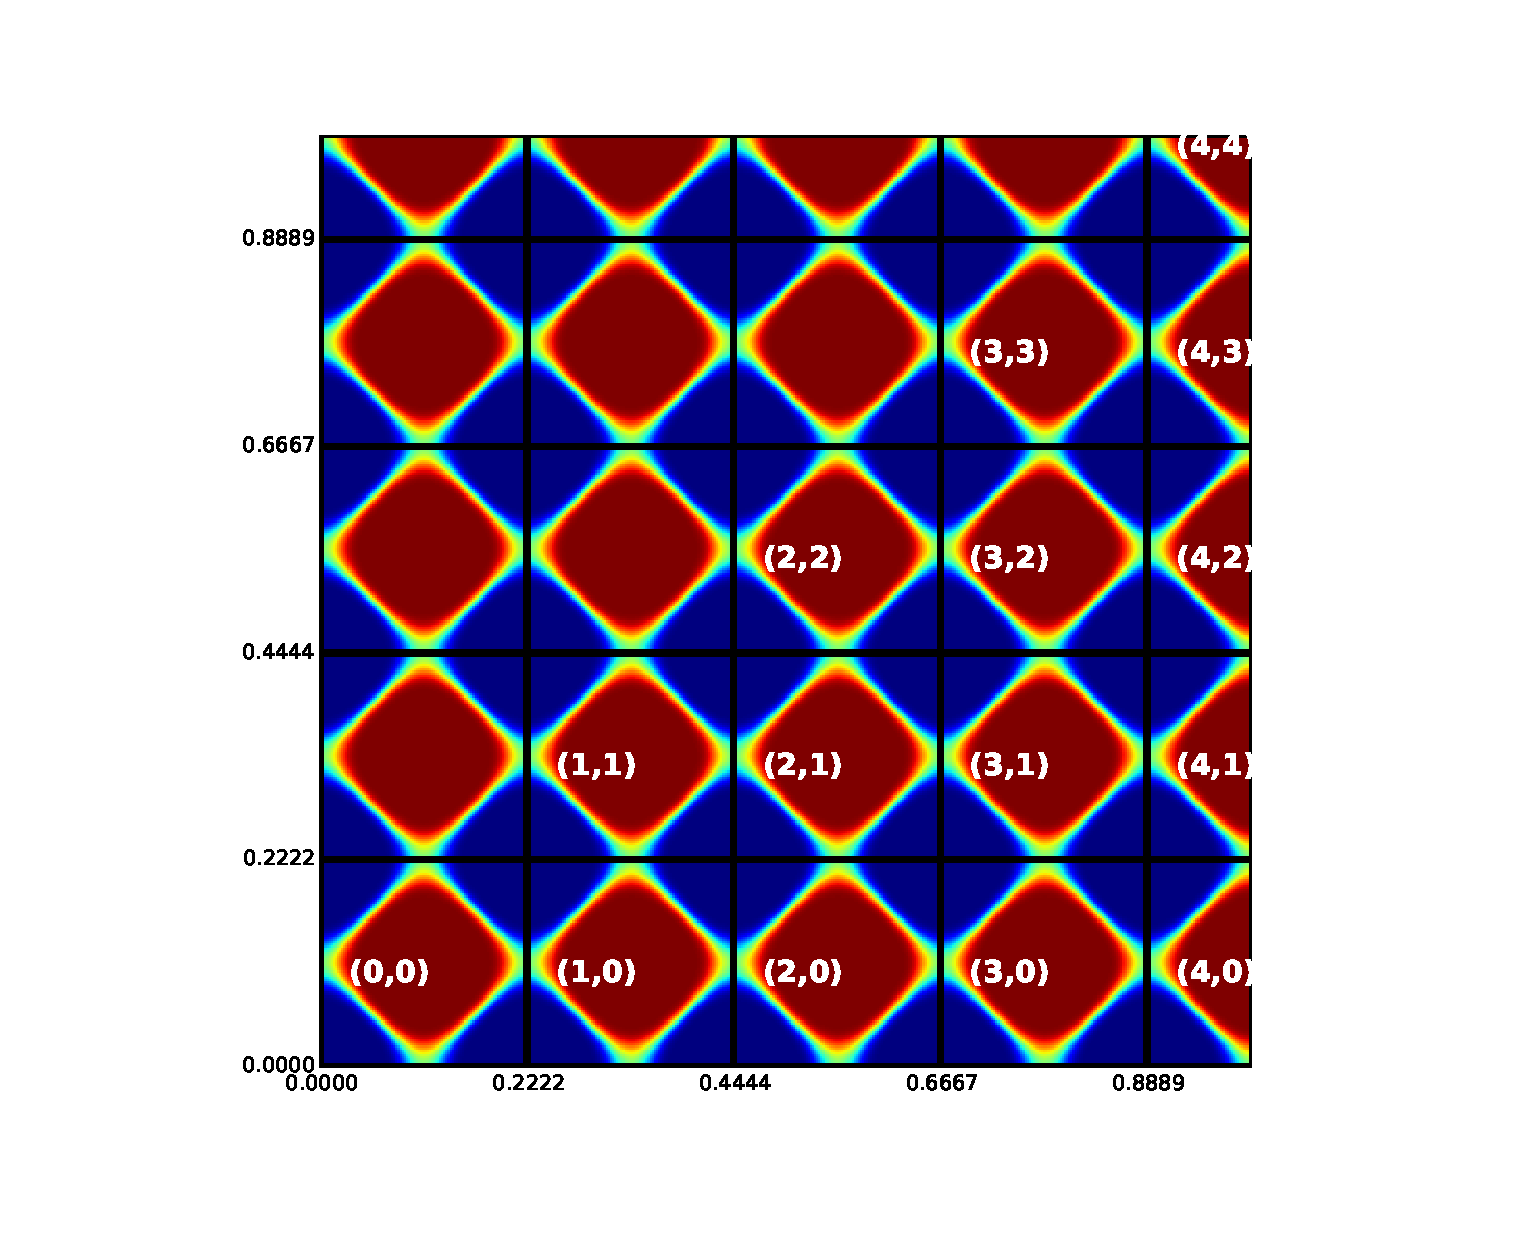
\includegraphics[width=\columnwidth]{figs/cells}
\caption{ \flabel{ic} 
Initial condition, $\phi(x,y,0,0)$, for 4.5 mode simulation.  
The bubbles are logically separated by the solid grid and each unique bubble is labeled.
}
\end{figure}

\begin{table}
\input{tbl/params.tbl}
\caption{ \tlabel{params}
Parameters of simulations.
The aspect ratio is defined with respect to the quiescent amplitude, $a_0$, from \eref{rollback}.
The last row is the simulation that extends the tank by a factor of two in the vertical direction.
}
\end{table}

Three simulations were conducted to reproduce experiments with 2.5, 3.5, and 4.5 modes across the diagonal.
Then, an extension of the 4.5 mode experiment with twice the vertical extent was performed.
Finally, a 4.5 mode calculation with periodic boundary conditions and unit Schmidt number was performed as a reference for comparing the growth of the bubbles in the wall-bounded flows.

The boundary conditions for the non-periodic simulations are no-slip for the velocity and no-flux (insulating) for the scalar.
The initial conditions for the velocity are quiescent.
The initial conditions for the scalar are the product of two cosines smeared by an error function in the z-direction:
\begin{equation}
  \phi(x,y,z,0) = \text{erf}\left[ \frac{z + a_0 \cos(k_x x) \cos(k_y y)}{\delta} \right] ,
\end{equation}
where $a_0$ is the initial amplitude,
$k_x$ and $k_y$ are the wave-numbers in the x and y directions, respectively, and
$\delta$ is the interface thickness.
In our case, $k_x = k_y$.
An example initial condition is plotted in \fref{ic}.
By symmetry, we know that the average scalar is zero, $H_{i,j} = H_{j,i}$, and that the spike dynamics are identical to the bubbles.

The Atwood number, local acceleration, and initial amplitude where taken from experimental measurements by Wilkinson and Jacobs~\cite{Wilkinson2007, JacobsPrivate}.
In the experiment, the interface has a non-zero initial velocity and the bulk flow is not measured.
Instead of trying to model the bulk flow, we used the linear theory, \eref{duff}, to transform the flow to quiescence.
Specifically, the system
\begin{align} \elabel{rollback}
H &= a_0 \cosh\left(\gamma (t - t_0)\right) \\
V &= a_0 \gamma \cosh\left(\gamma (t-t_0) \right)  \nonumber
\end{align}
where $H$ and $V$ were the experimental measures of the initial interface height and velocity, respectively,
is solved for $a_0$ and $t_0$, the quiescent amplitude and time.
The quiescent amplitude is used for the simulations.
The experiments to reproduce were selected such that solutions to \eref{rollback} existed and the bubble reached the greatest heights.

The viscosity is matched to the experimental fluids, but the diffusivity is not.
The Schmidt number in the experiments is in excess of 1000.
The computational cost of the simulation goes with the Schmidt number to the 4th power, so directly simulating such high Schmidt number was not possible.
Instead, the Schmidt number was varied in the range of 1 to 7 to gain a qualitative understanding of its influence on the flow.

It should be noted that, while the Atwood number was used to scale the local acceleration, the Boussinesq approximation implies that the Atwood number has been taken to zero while keeping the product $Ag$ fixed.
The generally accepted Boussinesq limit is $A = 0.05$, which is three times smaller than the Atwood number in this case.
Previous simulations directed at single-mode re-acceleration have been performed at $A \ge 0.15$, so it is not known whether re-acceleration persists in the limit as $A \rightarrow 0$.

The three simulations reproducing experimental runs are conducted on the Mira supercomputer at Argonne Leadership Computing Facility (ALCF).
The resolution and time-step was chosen to numerical stability constraints: a $256\times256\times512$ mesh of 7th order elements for 11,509,170,176 degrees of freedom.
The simulation was distributed over 524,288 cores and 1,048,576 MPI processes.
64 outputs were written to disk, each 6/8ths of a TiB.
The number of elements and degrees of freedom are doubled for the extension to twice the vertical extent.

\subsection{Post-processing}
The simulation outputs the velocity, pressure, and scalar fields at the Gauss-Lobatto-Legendre points in double precision.
They are post-processed into low-dimensional observables: the bubble height and two-dimensional slices of the velocity, vorticity, pressure, and scalar through the horizontal mid-plane and vertical diagonal.
Post-processing is performed using the `nek-analyze' post-processing framework, which implements a MapReduce-like backend for parallel, out-of-core analysis.

The bubble height is defined as:
\begin{equation} \elabel{h_exp}
H = \sup \left\{ z : \min_{x,y} \phi(x,y,z) < 0\right\},
\end{equation}
which, avoids measuring the diffusive growth by tracking the center of the interface profile instead of the ends.
The bubble velocity is found by fitting a cubic spline to $H(t)$ and differentiating.

The height of individual bubbles, $H_{i,j}$, is found by restricting $\min_{x,y}$ in \eref{h_exp} to the span-wise square of diagonal length $\lambda$ centered on the bubble in the $i$-by-$j$-th position.
The bubble domains and labels are shown in \fref{ic}.

